\documentclass{article}
\usepackage{amsmath,amssymb}
\usepackage[numbers]{natbib}
\usepackage{geometry}
 \geometry{
 a4paper,
 total={170mm,257mm},
 left=30mm,
 top=30mm,
 right=30mm,
 bottom=30mm
 }
 
\usepackage{graphicx}
\usepackage{caption}
\usepackage{subcaption}
\usepackage{float}

\usepackage{hyperref}
\hypersetup{%
  colorlinks=true,% hyperlinks will be coloured
}

\setlength{\parskip}{1em}

\title{Reinforcement Learning Assignment-4 \\
	\Large Model-Free Prediction and Control \\}
\begin{document}
\author{Utkarsh Prakash \\ \normalsize 180030042}
\maketitle
\section{MountainCar}
A car is on a one-dimensional track, positioned between two "mountains". The goal is to drive up the mountain on the right; 
however, the car's engine is not strong enough to scale the mountain in a single pass. Therefore, the only way to succeed is to 
drive back and forth to build up momentum. \par

\noindent %The next paragraph is not indented
The state of the car is decided by the position of the car along the horizontal axis and the velocity. At the beginning of the
episode, the car starts from the bottom of the hills (valley). The episode ends when the car reaches the goal or after
200 steps (which ever is earlier). The action space consists of 3 actions: \{push left, push right, do nothing\}. A negative reward
of $-1$ is applied at each timestep. The objective of the car is to reach the top of the hill on the right as early as possible, 
because at each timestep it will be rewarded negatively. \par

\begin{figure}[H]
    \graphicspath{ {../tmp/} }
    \begin{center}
    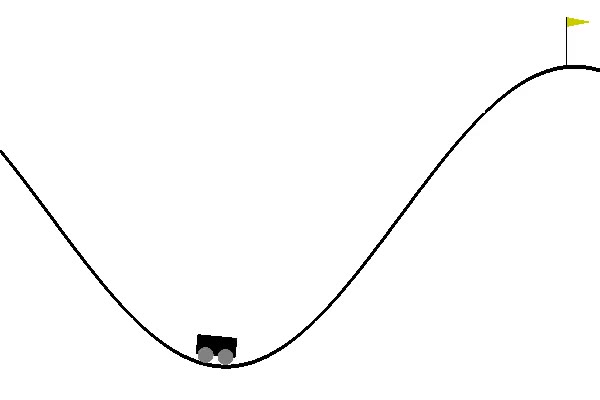
\includegraphics[width=8cm]{mountain_car.jpg}
    \end{center}
    \caption{MountainCar. For more details click \href{https://gym.openai.com/envs/MountainCar-v0/}{here} }
    \label{policy_iter_jack_problem}
\end{figure}

\noindent %The next paragraph is not indented
We compare the performance of Monte Carlo method, SARSA and Q-Learning algorithms on the Mountain Car problem. However, in order to
apply these algorithms we first need to discretize the state space. In order to do so, we round the position of the car to the nearest
$0.1$ and the velocity of the car to the nearest $0.01$. We also multiply the position and velocity of the car by $10$ and $100$ 
respectively, for convenience. \par

\noindent %The next paragraph is not indented
We run each of the algorithm for $20,000$ episodes and average the results over $10$ runs. The $\epsilon$ or the exploration factor
in the $\epsilon$-greedy policy is chosen to be $0.8$ initially and is decreased by a factor of $0.99$ after every epsiode. This ensures
that each of the state is explored infinitely often. The learning rate or the step-size $(\alpha)$ and discount factor $(\gamma)$ are 
chosen to $0.02$ and $0.9$ respectively. We use a constant step-size. The results obtained are as follows:\par

\begin{figure}[H]
    \graphicspath{ {../experiments/MountainCar/} }
    \centering
    \begin{minipage}{.5\textwidth}
      \centering
      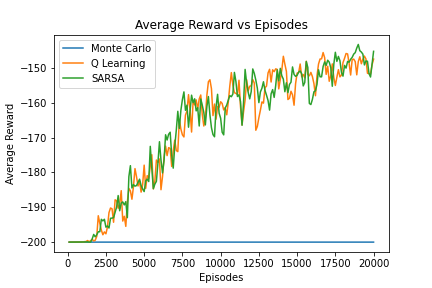
\includegraphics[width=\linewidth]{Mountaincar.png}
      \captionof{figure}{Average reward as a function of episode for MountainCar}
      \label{fig:test1}
    \end{minipage}%
    \begin{minipage}{.5\textwidth}
      \centering
      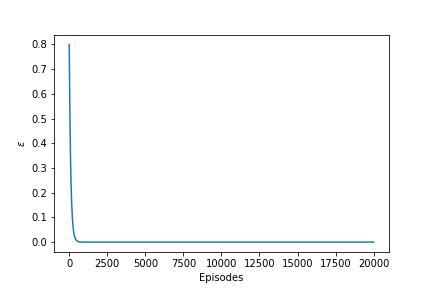
\includegraphics[width=\linewidth]{Mountaincar_epsilon.png}
      \captionof{figure}{$\epsilon$ as a function of episode for MountainCar}
      \label{fig:test2}
    \end{minipage}
    \end{figure}

    \begin{figure}[H]
        \graphicspath{ {../experiments/MountainCar/} }
        \centering
        \begin{minipage}{.33\textwidth}
        \nonumber
          \centering
          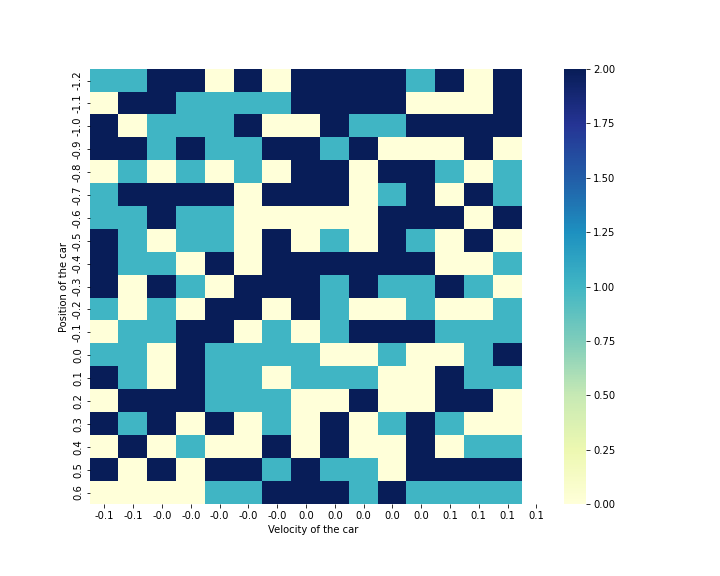
\includegraphics[width=\linewidth]{Mountaincar_montecarlo_policy.png}
          \captionof{figure}{Monte Carlo}
          \label{fig:test1}
        \end{minipage}%
        \begin{minipage}{.33\textwidth}
        \nonumber
          \centering
          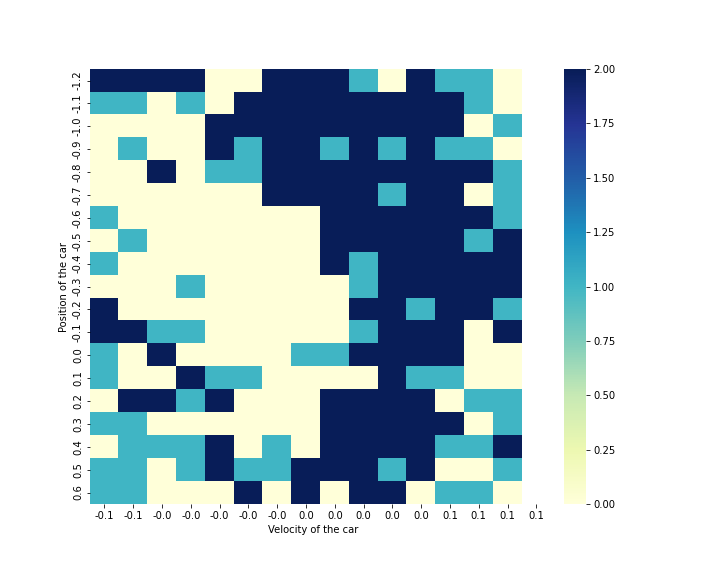
\includegraphics[width=\linewidth]{Mountaincar_sarsa_policy.png}
          \captionof{figure}{SARSA}
          \label{fig:test2}
        \end{minipage}
        \begin{minipage}{.33\textwidth}
        \nonumber
            \centering
            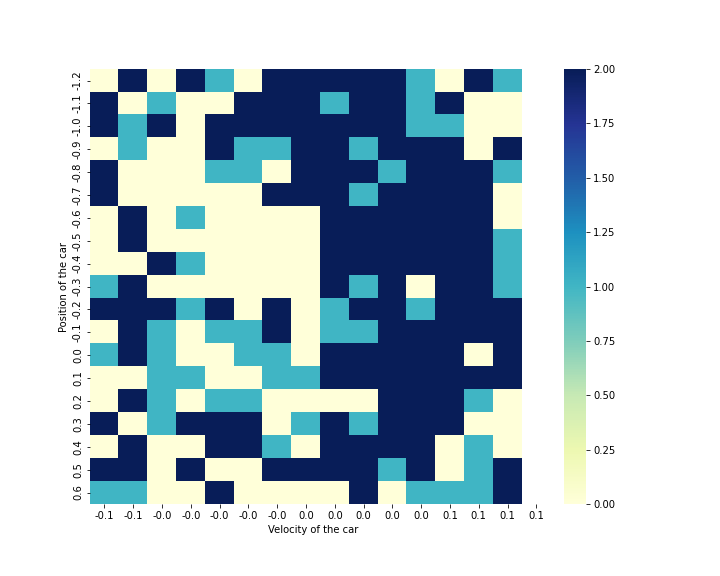
\includegraphics[width=\linewidth]{Mountaincar_qlearn_policy.png}
            \captionof{figure}{Q-Learning}
            \label{fig:test2}
          \end{minipage}
        \captionof{figure}{Final Policy for MountainCar learned by different algorithms for one of the runs. Action $0$ (light yellow) represents
        "push left", Action $1$ (light blue) represents "do nothing" and Action $2$ (dark blue) represents "push right".}
        \end{figure}

\noindent %The next paragraph is not indented
We can observe that Q-learning and SARSA algorithm perform equally well for the MountainCar problem. However, Monte Carlo methods
perform very bad on the MountainCar problem even after $20,000$ episodes. 

\section{Cart Pole}
A pole is attached by an un-actuated joint to a cart, which moves along a frictionless track. The system is controlled by applying a 
force of +1 or -1 to the cart. The pendulum starts upright, and the goal is to prevent it from falling over. A reward of +1 is provided for
every timestep that the pole remains upright. The episode ends when the pole is more than 15 degrees from vertical, or the cart moves more 
than 2.4 units from the center or the length of the episode is atleast 200.\par

\begin{figure}[H]
    \graphicspath{ {../tmp/} }
    \begin{center}
    
\includegraphics[width=8cm]{cartpole.png}
    \end{center}
    \caption{CartPole. For more details click \href{https://gym.openai.com/envs/CartPole-v1/}{here} }
    \label{policy_iter_jack_problem}
\end{figure}

\noindent %The next paragraph is not indented
The state of the cart is decided by it's position (x), velocity (x\_dot), pole angle (theta) and pole angular velocity (theta\_dot). The action space
consists of 2 actions: \{push left, push right\}.\par

\noindent %The next paragraph is not indented
We compare the performance of Monte Carlo method, SARSA and Q-Learning algorithms on the Mountain Car problem. However, in order to
apply these algorithms we first need to discretize the state space. For simiplicity, we discretize only the pole angle (theta) and pole angular velocity
(theta\_dot) space into $50$ equal-sized bins. Moreover, we also considering angular velocity $\in [-0.87, 0.87]$.\par

\noindent %The next paragraph is not indented
We run each of the algorithm for $20,000$ episodes and average the results over $10$ runs. The $\epsilon$ or the exploration factor
in the $\epsilon$-greedy policy is chosen to be $0.8$ initially and is decreased by a factor of $0.9999$ after every epsiode. This ensures
that each of the state is explored infinitely often. The learning rate or the step-size $(\alpha)$ and discount factor $(\gamma)$ are 
chosen to $0.2$ and $0.9$ respectively. We use a constant step-size. The results obtained are as follows:\par

\begin{figure}[H]
    \graphicspath{ {../experiments/CartPole/} }
    \centering
    \begin{minipage}{.5\textwidth}
      \centering
      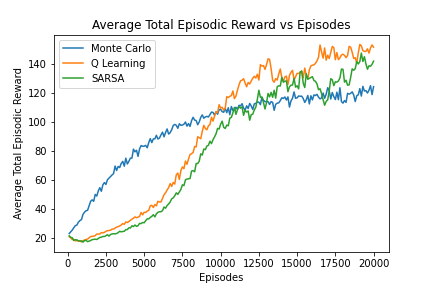
\includegraphics[width=\linewidth]{CartPole.png}
      \captionof{figure}{Average reward as a function of episode for CartPole}
      \label{fig:test1}
    \end{minipage}%
    \begin{minipage}{.5\textwidth}
      \centering
      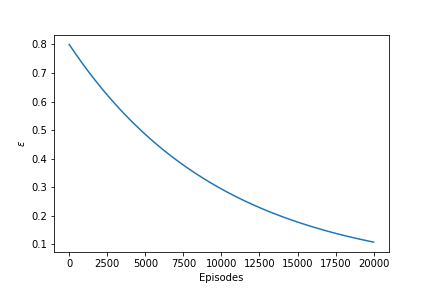
\includegraphics[width=\linewidth]{Cartpole_epsilon.png}
      \captionof{figure}{$\epsilon$ as a function of episode for CartPole}
      \label{fig:test2}
    \end{minipage}
    \end{figure}

    \begin{figure}[H]
        \graphicspath{ {../experiments/CartPole/} }
        \centering
        \begin{minipage}{.33\textwidth}
        \nonumber
          \centering
          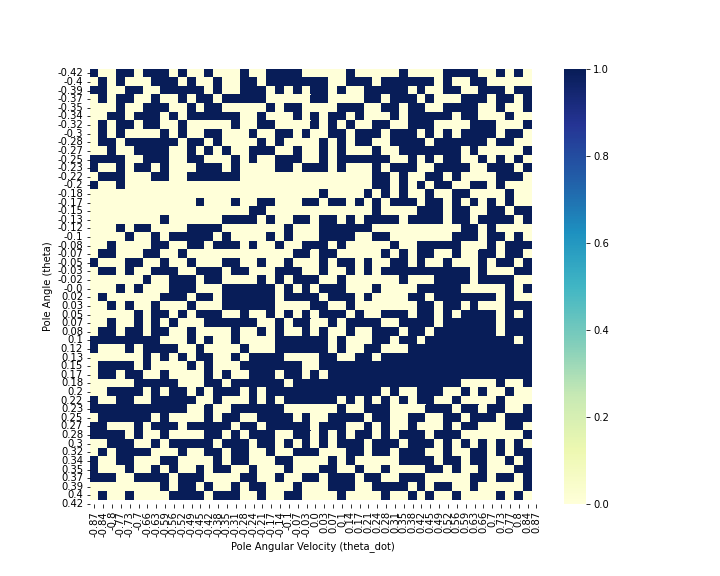
\includegraphics[width=\linewidth]{CartPole_montecarlo_policy.png}
          \captionof{figure}{Monte Carlo}
          \label{fig:test1}
        \end{minipage}%
        \begin{minipage}{.33\textwidth}
        \nonumber
          \centering
          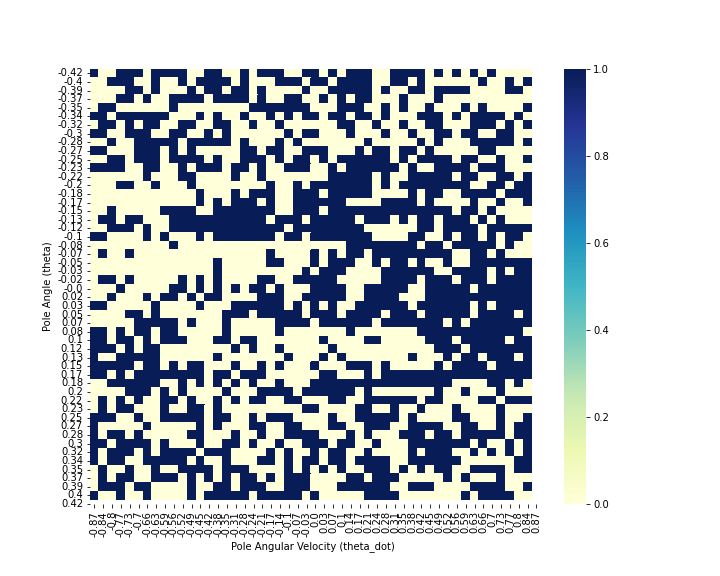
\includegraphics[width=\linewidth]{CartPole_sarsa_policy.png}
          \captionof{figure}{SARSA}
          \label{fig:test2}
        \end{minipage}
        \begin{minipage}{.33\textwidth}
        \nonumber
            \centering
            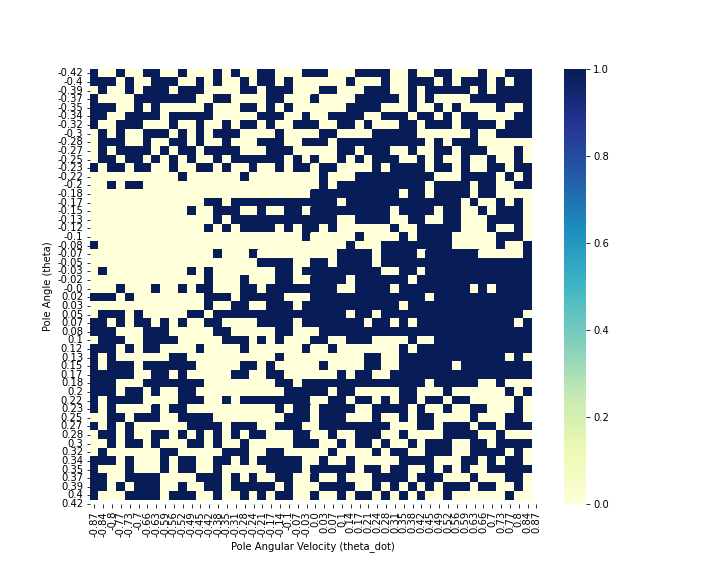
\includegraphics[width=\linewidth]{CartPole_qlearn_policy.png}
            \captionof{figure}{Q-Learning}
            \label{fig:test2}
          \end{minipage}
        \captionof{figure}{Final Policy for CartPole learned by different algorithms for one of the runs. Action $0$ (light yellow) represents
        "push left", Action $1$ (dark blue) represents "push right".}
        \end{figure}

\noindent %The next paragraph is not indented
We observe that Q-learning algorithm performs the best. The performance of SARSA algorithm is also comparable to that of Q-learning.
However, Monte Carlo methods perform much better this time. We observe that initially, Monte Carlo plots have higher wiggles than
Q-learning and SARSA, which can be attributed to the fact that Monte Carlo estimates have higher variance than its counterparts. 
On the other hand, Monte Carlo due its lower bias is initially able to learn quickly.

\end{document}